\documentclass[otchet]{SCWorks}
% Тип обучения (одно из значений):
%    bachelor   - бакалавриат (по умолчанию)
%    spec       - специальность
%    master     - магистратура
% Форма обучения (одно из значений):
%    och        - очное (по умолчанию)
%    zaoch      - заочное
% Тип работы (одно из значений):
%    coursework - курсовая работа (по умолчанию)
%    referat    - реферат
%  * otchet     - универсальный отчет
%  * nirjournal - журнал НИР
%  * digital    - итоговая работа для цифровой кафдры
%    diploma    - дипломная работа
%    pract      - отчет о научно-исследовательской работе
%    autoref    - автореферат выпускной работы
%    assignment - задание на выпускную квалификационную работу
%    review     - отзыв руководителя
%    critique   - рецензия на выпускную работу
% Включение шрифта
%    times      - включение шрифта Times New Roman (если установлен)
%                 по умолчанию выключен
\usepackage{preamble}
% \captionsetup[figure]{font= normalsize, labelfont=normalsize}
\renewcommand\theFancyVerbLine{\small\arabic{FancyVerbLine}}

\begin{document}

% Кафедра (в родительном падеже)
\chair{математической кибернетики и компьютерных наук}

% Тема работ
\title{Моделирование}

% Курс
\course{4}

% Группа
\group{451}

% Факультет (в родительном падеже) (по умолчанию "факультета КНиИТ")
% \department{факультета КНиИТ}

% Специальность/направление код - наименование
% \napravlenie{02.03.02 "--- Фундаментальная информатика и информационные технологии}
% \napravlenie{02.03.01 "--- Математическое обеспечение и администрирование информационных систем}
% \napravlenie{09.03.01 "--- Информатика и вычислительная техника}
\napravlenie{09.03.04 "--- Программная инженерия}
% \napravlenie{10.05.01 "--- Компьютерная безопасность}

% Для студентки. Для работы студента следующая команда не нужна.
% \studenttitle{Студентки}

% Фамилия, имя, отчество в родительном падеже
\author{Устюшина Богдана Антоновича}

% Заведующий кафедрой 
\chtitle{доцент, к.\,ф.-м.\,н.}
\chname{С.\,В.\,Миронов}

% Руководитель ДПП ПП для цифровой кафедры (перекрывает заведующего кафедры)
% \chpretitle{
%     заведующий кафедрой математических основ информатики и олимпиадного\\
%     программирования на базе МАОУ <<Ф"=Т лицей №1>>
% }
%\chtitle{г. Саратов, к.\,ф.-м.\,н., доцент}
% \chname{Кондратова\, Ю.\,Н.}

% Научный руководитель (для реферата преподаватель проверяющий работу)
\satitle{доцент, к.\,ф.-м.\,н.} %должность, степень, звание
\saname{И.\,Е.\,Тананко}

% Руководитель практики от организации (руководитель для цифровой кафедры)
\patitle{доцент, к.\,ф.-м.\,н.}
\paname{С.\,В.\,Миронов}

% Руководитель НИР
\nirtitle{доцент, к.\,п.\,н.} % степень, звание
\nirname{В.\,А.\,Векслер}

% Семестр (только для практики, для остальных типов работ не используется)
\term{6}

% Наименование практики (только для практики, для остальных типов работ не
% используется)
\practtype{производственная}

% Продолжительность практики (количество недель) (только для практики, для
% остальных типов работ не используется)
\duration{4}

% Даты начала и окончания практики (только для практики, для остальных типов
% работ не используется)
\practStart{01.08.2024}
\practFinish{28.08.2024}

% Год выполнения отчета
\date{2025}

\maketitle

% Включение нумерации рисунков, формул и таблиц по разделам (по умолчанию -
% нумерация сквозная) (допускается оба вида нумерации)
% \secNumbering

% \tableofcontents

% Раздел "Обозначения и сокращения". Может отсутствовать в работе
% \abbreviations
% \begin{description}
%     \item ... "--- ...
%     \item ... "--- ...
% \end{description}

% Раздел "Определения". Может отсутствовать в работе
% \definitions

% Раздел "Определения, обозначения и сокращения". Может отсутствовать в работе.
% Если присутствует, то заменяет собой разделы "Обозначения и сокращения" и
% "Определения"
% \defabbr

\sloppy

\intro

Отчёт по предмету моделирование. Всего выполнено 6 заданий: для каждого из них
построена математическая модель. Затем на языке программирования Python 
произведено моделирование с определёнными параметрами, заданными заранее.

Порядковый номер в группе — 15, соответственно все выполненные задачи — пятнадцатые
в списке.

\section{Моделирование непрерывных систем}

\subsection{Дифференциальные уравнения первого порядка}

\textbf{Задание}

\begin{figure}[H]
	\center{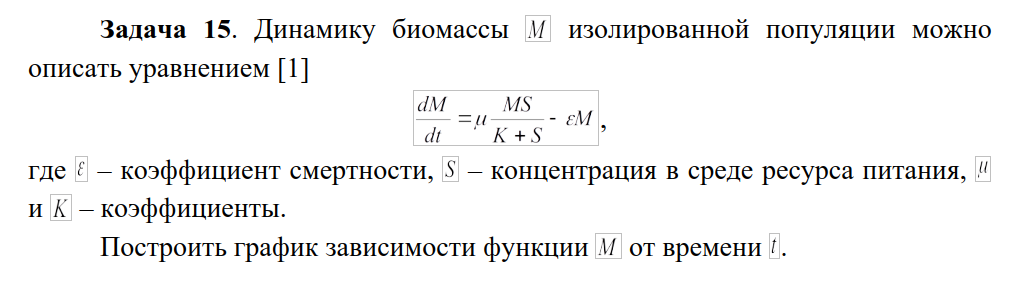
\includegraphics[scale=0.47]{pics/task1.png}}
	\caption{Задание 1.1}
	\label{pic1}
\end{figure}

\textbf{Решение} представлено в приложении \ref{ap_task1_1}

\textbf{Результат}

\begin{figure}[H]
	\center{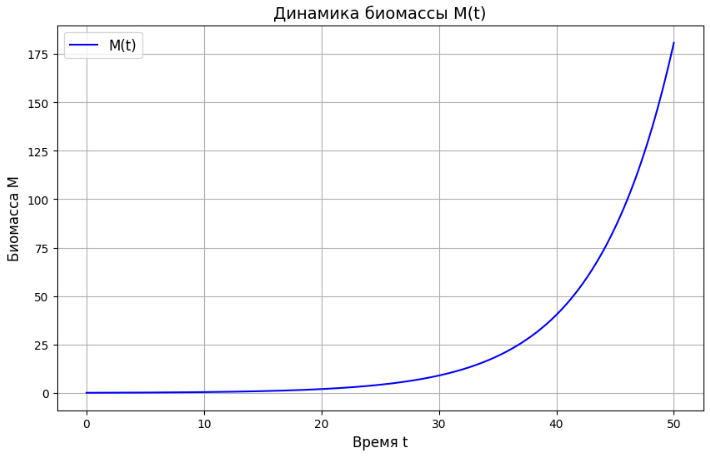
\includegraphics[scale=0.6]{pics/res_1.png}}
	\caption{График решения задания 1.1}
	\label{res1}
\end{figure}

\subsection{Системы дифференциальных уравнений}

\textbf{Задание}

\begin{figure}[H]
	\center{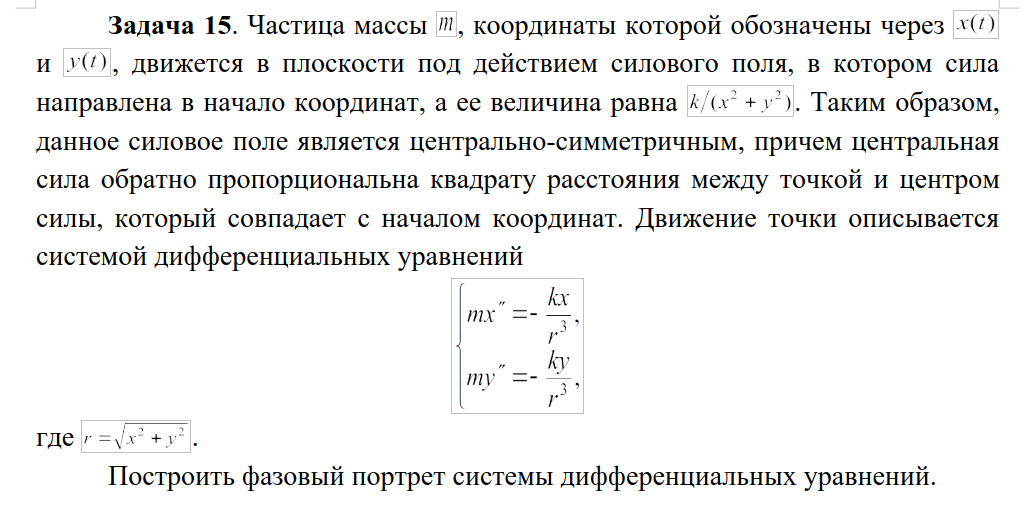
\includegraphics[scale=0.47]{pics/task2.png}}
	\caption{Задание 1.2}
	\label{pic2}
\end{figure}

\textbf{Решение} представлено в приложении \ref{ap_task1_2}

\textbf{Результат}

\begin{figure}[H]
	\center{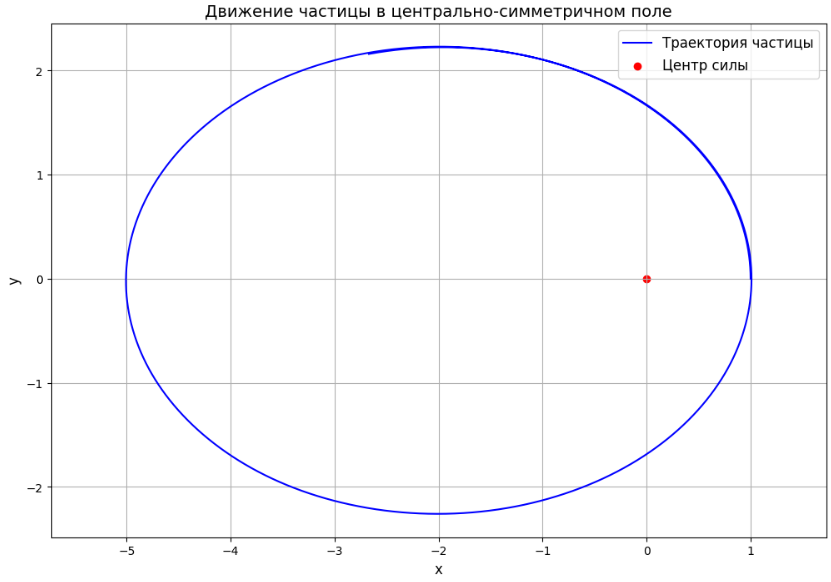
\includegraphics[scale=0.6]{pics/res_2.png}}
	\caption{График решения задания 1.2}
	\label{res2}
\end{figure}

\section{Метод статистических испытаний}

\subsection{Равномерно распределённая дискретная случайная величина}

\textbf{Задание}

\begin{figure}[H]
	\center{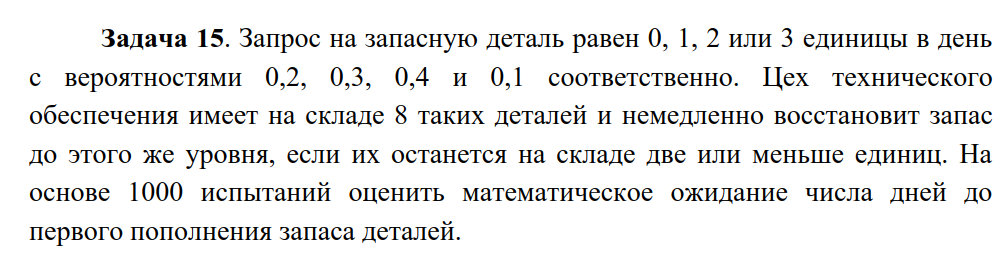
\includegraphics[scale=0.6]{pics/task3.png}}
	\caption{Задание 2.1}
	\label{pic3}
\end{figure}

\textbf{Решение} представлено в Приложении \ref{ap_task2_1}

\textbf{Результат} 

Оценка математического ожидания числа дней до первого пополнения: 4.71

\subsection{Равномерно распределённая непрерывная случайная величина}

\textbf{Задание}

\begin{figure}[H]
	\center{
\includegraphics[scale=0.6]{pics/task4.png}}
	\caption{Задание 2.2}
	\label{pic4}
\end{figure}

\textbf{Решение} представлено в Приложении \ref{ap_task2_2}

\textbf{Результат} 

Оцененная вероятность ожидания: 0.1195

\subsection{Нормально распределённая случайная величина}

\textbf{Задание}

\begin{figure}[H]
	\center{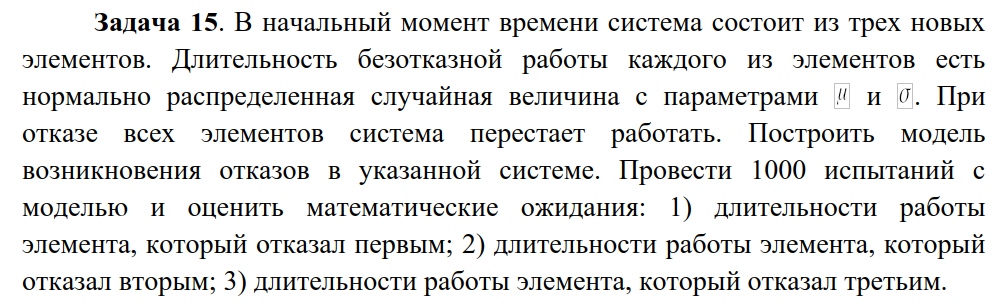
\includegraphics[scale=0.6]{pics/task5.png}}
	\caption{Задание 2.3}
	\label{pic5}
\end{figure}

\textbf{Решение} представлено в Приложении \ref{ap_task2_3}

\textbf{Результат}

Математическое ожидание длительности работы элемента, отказавшего первым: 87.62

Математическое ожидание длительности работы элемента, отказавшего вторым: 100.27

Математическое ожидание длительности работы элемента, отказавшего третьим: 112.84

\subsection{Экспоненциально распределённая случайная величина}

\textbf{Задание}

\begin{figure}[H]
	\center{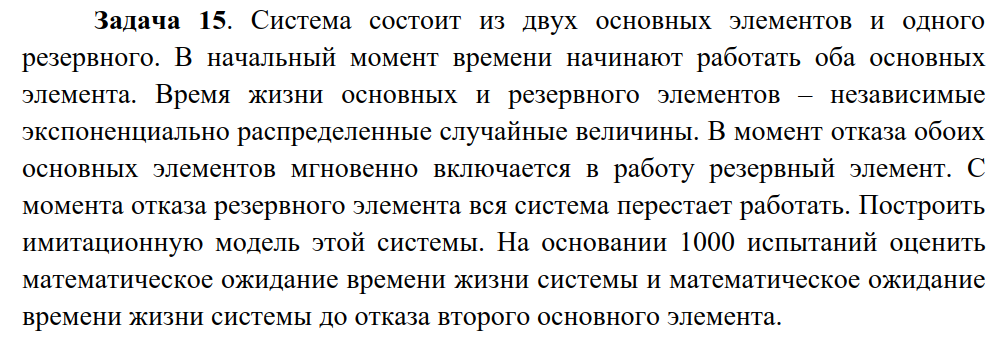
\includegraphics[scale=0.6]{pics/task6.png}}
	\caption{Задание 2.4}
	\label{pic6}
\end{figure}

\textbf{Решение} представлено в Приложении \ref{ap_task2_4}

\textbf{Результат} 

Математическое ожидание времени жизни системы: 298.75

Математическое ожидание времени жизни системы до отказа второго основного элемента: 150.35

\section{Метод статистических испытаний}
\subsection{Равномерно распределённая дискретная случайная величина}

\textbf{Задание}

\begin{figure}[H]
	\center{
\includegraphics[scale=0.3]{pics/task7.png}}
	\caption{Задание 3.1}
	\label{pic7}
\end{figure}

\textbf{Решение} представлено в Приложении \ref{ap_task3_1}

\textbf{Результат} 

Результаты моделирования (на основе 1000 поступлений):

\underline{Класс 1:} 

Всего поступило = 407, $\overline{u}_1$ (ср. время пребывания) = 0.298

\underline{Класс 2:}

Всего поступило = 593, $\overline{u}_2$ = 0.792

Вероятность отказа = 0.292

\underline{Общее модельное время:} 208.852

\appendix
\section{Решения раздела 1}
\subsection{Задание 1.1}
\label{ap_task1_1}
\begin{minted}[linenos, breaklines=true, style=bw]{Python}
import numpy as np
import matplotlib.pyplot as plt
from scipy.integrate import solve_ivp
mu = 0.5
K = 1.0 
eps = 0.1
S = 1.0 
M0 = 0.1
t_span = (0, 50) 
t_eval = np.linspace(t_span[0], t_span[1], 500) 
def biomass_dynamics(t, M):
    return mu * (M * S) / (K + S) - eps * M
solution = solve_ivp(biomass_dynamics, t_span, [M0], t_eval=t_eval)
plt.figure(figsize=(10, 6))
plt.plot(solution.t, solution.y[0], label="M(t)", color="blue")
plt.title("Динамика биомассы M(t)", fontsize=14)
plt.xlabel("Время t", fontsize=12)
plt.ylabel("Биомасса M", fontsize=12)
plt.grid(True)
plt.legend(fontsize=12)
plt.show()
\end{minted}

\subsection{Задание 1.2}
\label{ap_task1_2}
\begin{minted}[linenos, breaklines=true, style=bw]{Python}
from scipy.integrate import solve_ivp
import matplotlib.pyplot as plt
import numpy as np
m = 1.0 
k = 1.0 
x0, y0 = 1.0, 0.0 
vx0, vy0 = 0.0, 1.0
t_span = (0, 50)  
t_eval = np.linspace(t_span[0], t_span[1], 10000) 
def central_force(t, state):
    x, y, vx, vy = state
    r = np.sqrt(x**2 + y**2) 
    ax = -k * x / r**3 
    ay = -k * y / r**3
    return [vx, vy, ax, ay]
initial_state = [x0, y0, vx0, vy0]
solution = solve_ivp(central_force, t_span, initial_state, t_eval=t_eval)
x, y = solution.y[0], solution.y[1]
plt.figure(figsize=(12, 8))
plt.plot(x, y, label="Траектория частицы", color="blue")
plt.scatter(0, 0, color="red", label="Центр силы")
plt.title("Движение частицы в центрально-симметричном поле", fontsize=14)
plt.xlabel("x", fontsize=12)
plt.ylabel("y", fontsize=12)
plt.grid(True)
plt.axis("equal")
plt.legend(fontsize=12)
plt.show()
\end{minted}

\section{Решения раздела 2}
\subsection{Задание 2.1}
\label{ap_task2_1}
\begin{minted}[linenos, breaklines=true, style=bw]{Python}
import numpy as np
probabilities = [0.2, 0.3, 0.4, 0.1] 
requests = [0, 1, 2, 3]
initial_stock = 8
threshold = 2 
num_trials = 1000 
def simulate_single_trial():
    stock = initial_stock
    days = 0
    while stock > threshold:
        daily_request = np.random.choice(requests, p=probabilities)
        stock -= daily_request
        stock = max(stock, 0) 
    days += 1
    return days
results = [simulate_single_trial() for _ in range(num_trials)]
expected_days = np.mean(results)
print(f"Оценка математического ожидания числа дней до первого пополнения: {expected_days:.2f}")
\end{minted}
\subsection{Задание 2.2}
\label{ap_task2_2}
\begin{minted}[linenos, breaklines=true, style=bw]{Python}
import numpy as np
time_range = 24 
ship1_stay = 1 
ship2_stay = 2 
num_trials = 100000 
def intervals_overlap(start1, duration1, start2, duration2):
    end1 = start1 + duration1
    end2 = start2 + duration2
    return not (end1 <= start2 or end2 <= start1)
conflict_count = 0
for _ in range(num_trials):
    arrival1 = np.random.uniform(0, time_range) 
    arrival2 = np.random.uniform(0, time_range) 
    if intervals_overlap(arrival1, ship1_stay, arrival2, ship2_stay):
        conflict_count += 1
probability = conflict_count / num_trials
print(f"Оцененная вероятность ожидания: {probability:.4f}")
\end{minted}
\subsection{Задание 2.3}
\label{ap_task2_3}
\begin{minted}[linenos, breaklines=true, style=bw]{Python}
import numpy as np
mean_lifetime = 100 
std_lifetime = 15    
num_trials = 1000    
def simulate_failure_times():
    lifetimes = np.random.normal(mean_lifetime, std_lifetime, 3)
    lifetimes.sort() 
    return lifetimes
first_failures = []
second_failures = []
third_failures = []
for _ in range(num_trials):
    lifetimes = simulate_failure_times()
    first_failures.append(lifetimes[0])
    second_failures.append(lifetimes[1])
    third_failures.append(lifetimes[2])
mean_first_failure = np.mean(first_failures)
mean_second_failure = np.mean(second_failures)
mean_third_failure = np.mean(third_failures)
print(f"Математическое ожидание длительности работы элемента, отказавшего первым: {mean_first_failure:.2f}")
print(f"Математическое ожидание длительности работы элемента, отказавшего вторым: {mean_second_failure:.2f}")
print(f"Математическое ожидание длительности работы элемента, отказавшего третьим: {mean_third_failure:.2f}")
\end{minted}
\subsection{Задание 2.4}
\label{ap_task2_4}
\begin{minted}[linenos, breaklines=true, style=bw]{Python}
import numpy as np
mean_lifetime_main = 100
mean_lifetime_reserve = 150
num_trials = 10000
def simulate_system_lifetime():
    main1 = np.random.exponential(mean_lifetime_main)
    main2 = np.random.exponential(mean_lifetime_main)
    reserve = np.random.exponential(mean_lifetime_reserve)
second_main_failure = max(main1, main2)
system_lifetime = second_main_failure + reserve
return system_lifetime, second_main_failure
system_lifetimes = []
second_main_failures = []
for _ in range(num_trials):
    system_lifetime, second_main_failure = simulate_system_lifetime()
    system_lifetimes.append(system_lifetime)
    second_main_failures.append(second_main_failure)
mean_system_lifetime = np.mean(system_lifetimes)
mean_second_main_failure = np.mean(second_main_failures)
print(f"Математическое ожидание времени жизни системы: {mean_system_lifetime:.2f}")
print(f"Математическое ожидание времени жизни системы до отказа второго основного элемента: {mean_second_main_failure:.2f}")    
\end{minted}

\section{Решения раздела 3}

\subsection{Задание 3.1}
\label{ap_task3_1}
\begin{minted}[linenos, breaklines=true, style=bw]{Python}
    import random
    # Параметры модели
    lambda1 = 2     
    lambda2 = 3     
    mu = 5.0      # интенсивность обслуживаний
    N = 1000      
    lambda_total = lambda1 + lambda2  # суммарная интенсивность поступлений
    t = 0.0 
    next_arrival = t + random.expovariate(lambda_total)
    # current_job - кортеж (job_class, arrival_time) для заявки, находящейся в обслуживании.
    current_job = None
    departure_time = float('inf') 
    # Очереди ожидания: для каждого класса храним кортеж (job_class, arrival_time)
    queue1 = []  # для требований 1-го класса
    queue2 = []  # для требований 2-го класса
    # Счётчики поступлений по классам
    total_arrivals = 0
    total_arrivals_class1 = 0
    total_arrivals_class2 = 0
    # Для расчёта математического ожидания времени пребывания (u)
    sum_sojourn_class1 = 0.0  # суммарное время пребывания для требований 1-го класса
    sum_sojourn_class2 = 0.0  # суммарное время пребывания для требований 2-го класса
    count_class1 = 0         
    count_class2 = 0         
    lost2_count = 0
    # Моделирование продолжается, пока не сгенерируем N поступлений и система не опустеет.
    while total_arrivals < N or current_job is not None or queue1 or queue2:
        # Определяем следующее событие: поступление или завершение обслуживания.
        # Если ещё поступления не исчерпаны, выбираем событие с минимальным временем.
        if total_arrivals < N:
            # Сравниваем время следующего поступления и время завершения обслуживания.
            if next_arrival <= departure_time:
                event_type = 'arrival'
                event_time = next_arrival
            else:
                event_type = 'departure'
                event_time = departure_time
        else:
            # Если поступлений больше не генерируем, остаются только события завершения обслуживания.
            event_type = 'departure'
            event_time = departure_time
    
        t = event_time
        # Обработка поступления: генерируем требование и определяем его класс
        if event_type == 'arrival':    
            total_arrivals += 1
            if random.random() < lambda1 / lambda_total:
                job_class = 'class1'
                total_arrivals_class1 += 1
            else:
                job_class = 'class2'
                total_arrivals_class2 += 1
    
            arrival_record = (job_class, t)
            # Обработка поступления в зависимости от состояния сервера:
            if current_job is None:
                # Если сервер свободен – начинаем обслуживание сразу.
                current_job = arrival_record
                departure_time = t + random.expovariate(mu)
            else:
                if job_class == 'class1':
                    # Требование 1-го класса имеет абсолютный приоритет.
                    if current_job[0] == 'class2':
                        # Прерываем обслуживание требования 2-го класса.
                        # Засчитываем время пребывания прерванного требования 2-го класса.
                        sojourn = t - current_job[1]
                        sum_sojourn_class2 += sojourn
                        count_class2 += 1
                        lost2_count += 1
                        # Начинаем обслуживание требования 1-го класса, поступившего в данный момент.
                        current_job = arrival_record
                        departure_time = t + random.expovariate(mu)
                    else:
                        # Если сервер занят требованием 1-го класса, поступившее требование идёт в очередь.
                        queue1.append(arrival_record)
                else:
                    # Требование 2-го класса: если сервер занят, добавляем в очередь.
                    queue2.append(arrival_record)
    
            # Планируем следующее поступление, если общее число поступлений меньше N
            if total_arrivals < N:
                next_arrival = t + random.expovariate(lambda_total)
            else:
                next_arrival = float('inf')
        else:
            # Обработка завершения обслуживания (departure)
            finished_job = current_job
            sojourn = t - finished_job[1]  # время пребывания в системе = t - время поступления
            if finished_job[0] == 'class1':
                sum_sojourn_class1 += sojourn
                count_class1 += 1
            else:
                sum_sojourn_class2 += sojourn
                count_class2 += 1
            # Выбор следующего требования для обслуживания:
            # Абсолютный приоритет имеет очередь требований 1-го класса.
            if queue1:
                current_job = queue1.pop(0)
                departure_time = t + random.expovariate(mu)
            elif queue2:
                current_job = queue2.pop(0)
                departure_time = t + random.expovariate(mu)
            else:
                current_job = None
                departure_time = float('inf')
    u1 = sum_sojourn_class1 / count_class1 if count_class1 > 0 else 0.0
    u2 = sum_sojourn_class2 / count_class2 if count_class2 > 0 else 0.0
    refusal_prob_class2 = lost2_count / total_arrivals_class2 if total_arrivals_class2 > 0 else 0.0
    # Вывод результатов моделирования
    print("Результаты моделирования (на основе {} поступлений):".format(N))
    print("Класс 1: Всего поступило = {}, u1 (ср. время пребывания) = {:.3f}".format(total_arrivals_class1, u1))
    print("Класс 2: Всего поступило = {}, u2 (ср. время пребывания) = {:.3f}, Вероятность отказа = {:.3f}"
          .format(total_arrivals_class2, u2, refusal_prob_class2))
    print("Общее модельное время: {:.3f}".format(t))    
\end{minted}
\end{document}
